\subsection{Big Trees and Random Subsets}
\begin{lstlisting}[language={},numbers=left,numberstyle=\tiny,frame=single,breaklines=true,postbreak=\mbox{\textcolor{red}{$\hookrightarrow$}\space}]
Frequency of appearance: [      0       0 2212058 1353200 2094475   22530 2690463  536110   91164]
Most frequent : 6
\end{lstlisting}

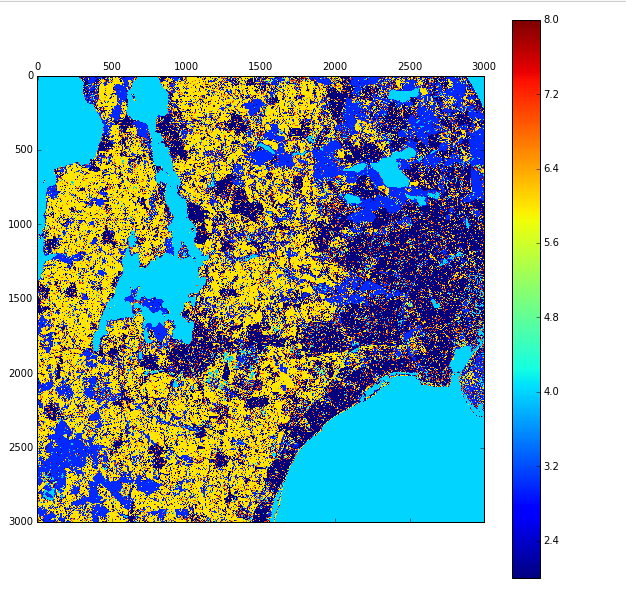
\includegraphics[width=10cm]{trees_pred.png}


\subsection{Runtime}
As stated on SKlearn's website, the runtime is $O()$
\subsection{Detecting Rare Instances}